
\begin{elevator}[Introduction to Surfaces]
We generalize our study of planar drawing to drawings on other surfaces, and along the way generalize our Euler's characteristic, and interpretations of planarity criterion. 
\label{sec:planar:surfaces}
\end{elevator}
The simplest kind of topological surface that we can look at are those of \emph{surfaces.} A good way to get an initial handle on surfaces is by describing them in terms of the combinatorial data of a graph drawn on that surface. We'll give a formal definition of a surface in the next section, but for now think of this as a shape without corners which you could make out of a rubber sheet.
\begin{definition}
An \emph{embedding} of a graph $G$ into a surface $\Sigma$ is a drawing of $G$ on $\Sigma$ where no edges cross eac hother. 
\end{definition}
Here are a few examples of embeddings of graphs into surfaces:

\begin{examplefigureenv}[Graph on the torus]{191figures/embgraph_graphOnTorus.tikz}
	Every planar graph embedding gives us an example of a surface embedding. A graph which is embeddable in the plane is embeddable in every surface, as each surface locally looks like a copy of the plane. Because of this, we see that one requires more than just the information of a graph on a surface to determine what surface we are looking at. 
\end{examplefigureenv}



\begin{examplefigureenv}[Stereographic Projection]{191figures/embgraph_stereographic.tikz}
	Graphs which are embeddable in the sphere are exactly equal to planar graphs. One can translate between these two types of graph via a technique called \emph{stereographic projection.}
\end{examplefigureenv}

\begin{examplefigureenv}[Differences in face counts]{191figures/embgraph_planeVsTorus.tikz}
	
There are of some more intesting graphs that we can embed on the torus. In the figure on the right, the graph drawn has only 1 face; but any planar drawing of this graph will have 3 faces as the graph has 2 cycles. 
\end{examplefigureenv}

\begin{comment}
It can be difficult to draw a graph on a surface when we imagine that surface being in 3-dimensional space-- especially when we consider that not every surface is embeddable in 3 dimensional space! Here is a convenient piece of notation or drawing technique for getting a better handle on visualizing surfaces. A \emph{gluing polygon} for a surface is a polygon where pairs of sides have been labeled with an orientation and letter. Such a diagram gives us a method for building a surface: imagine that this polygon was a sheet of rubber, and take pairs of sides equipped with the same label and glue them together as specified by the orientation. 
\begin{claim}
For any surface $\Sigma$, there exists a gluing polygon that glues up to that surface. 
\end{claim}
However, it is not the case that a gluing polygon uniquely determines a surface. 

\examplefigure{The torus has a nice description via a gluing polygon. When you take the sides labeled $a$ and glue them together, you get a cylinder. Then taking the top and bottom of the cylinder (labeled $b$) and bring them together folds this into a torus. }{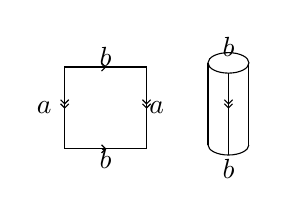
\begin{tikzpicture}[scale=.26]
\draw  (-2,2) rectangle (2,-2);
\draw (5.8,0.4) -- (6,0.2) -- (6.2,0.4);
\draw (5.8,0.2) -- (6,0) -- (6.2,0.2);
\draw (1.8,0.4) -- (2,0.2) -- (2.2,0.4);
\draw (1.8,0.2) -- (2,0) -- (2.2,0.2);
\draw (-0.2,2.2) -- (0,2) -- (-0.2,1.8);
\draw (-0.2,-1.8) -- (0,-2) -- (-0.2,-2.2);
\draw (-2.2,0.4) -- (-2,0.2) -- (-1.8,0.4);
\draw (-2.2,0.2) -- (-2,0) -- (-1.8,0.2);
\draw  (6,2.2) ellipse (1 and 0.5);
\draw  (6,-1.8) ellipse (1 and 0.5);
\fill[white]  (4.5,-0.8) rectangle (7.5,-1.8);
\draw (5,2.2) -- (5,-1.8);
\draw (7,2.2) -- (7,-1.8);
\draw (6,1.7) -- (6,-2.3);
\node at (-3,0) {$a$};
\node at (2.5,0) {$a$};
\node at (0,2.5) {$b$};
\node at (0,-2.5) {$b$};
\node at (6,3) {$b$};
\node at (6,-3) {$b$};
\end{tikzpicture}}
It is in general a lot easier to draw a graph on a gluing polygon than it is to draw it in the plane. See Figure \ref{fig:k33torus} for an example of $K_{3,3}$ drawn on the torus via a gluing diagram. 
\begin{wrapfigure}{l}{5cm}
\centering
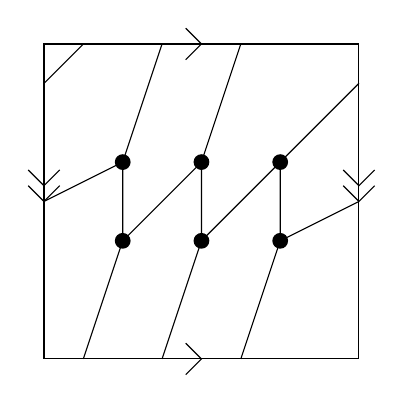
\begin{tikzpicture}
\draw  (-2,2) rectangle (2,-2);
\draw (-2.2,0.4) -- (-2,0.2) -- (-1.8,0.4);
\draw (-2.2,0.2) -- (-2,0) -- (-1.8,0.2);
\draw (1.8,0.4) -- (2,0.2) -- (2.2,0.4);
\draw (1.8,0.2) -- (2,0) -- (2.2,0.2);
\draw (-0.2,2.2) -- (0,2) -- (-0.2,1.8);
\draw (-0.2,-1.8) -- (0,-2) -- (-0.2,-2.2);
\fill (1,0.5) circle[radius=.1];
\fill (1,-0.5) circle[radius=.1];
\fill (0,0.5) circle[radius=.1];
\fill (0,-0.5) circle[radius=.1];
\fill (-1,-0.5) circle[radius=.1];
\fill (-1,0.5) circle[radius=.1];
\draw (-1,0.5) -- (-1,-0.5) -- (0,0.5) -- (0,-0.5) -- (1,0.5) -- (1,-0.5);
\draw (0,0.5) -- (0.5,2);
\draw (0.5,-2) -- (1,-0.5);
\draw (0,-0.5) -- (-0.5,-2);
\draw (-0.5,2) -- (-1,0.5);
\draw (-1,0.5) -- (-2,0);
\draw (2,0) -- (1,-0.5);
\draw (1,0.5) -- (2,1.5);
\draw (-2,1.5) -- (-1.5,2);
\draw (-1.5,-2) -- (-1,-0.5);
\end{tikzpicture}
\caption{$K_{3,3}$ on the Torus}
\label{fig:k33torus}
\end{wrapfigure}

We  noticed in our first example, that not every graph gives us a good interpretation of a surface.  
\begin{definition}
A graph embedding $G$ provides a \emph{net} of surface $\Sigma$ if $\Sigma\setminus G$ has only contractible connected components. As in the case of planar graphs, we call each connected component a \emph{face}. 
\end{definition}
Notice that a graph can be a net for many different surfaces, provided that we do not remember the data of which parts of the net bound faces.  \\
As in the case with planar graphs, it becomes interesting to study the alternating sum of the different strata that a graph decomposes a surface into. 
\begin{definition}
Let $G$ be a net for a surface $\Sigma$. We define that the \emph{Euler Characteristic} of the net to be the alternating sum
\[\chi_G(\Sigma):= |V|-|E|+|F|.\]
\end{definition}
In the case of a planar graph, we always get a net, and thus the Euler characteristic of any planar net is 2. However, the Euler characteristic is different as we vary surface. 

\examplefigure{Here is a non-example and an example of a net for the torus.\\
In the first drawing, removing the triangle separates the torus into 2 connected components. The first one looks like the bounded triangle. The remainder of the torus stays largely intact after this operation. The remaining surface looks like a ``torus with a puncture.''\\
In the second drawing, the removal of the graph results in a single connected component that looks like a square. To see this, take the 4 squares that are drawn, and glue them together by the rules ascribed by the edges. The resulting glued together shape is, once again, a square, which is contractible. The number of vertices in this example is 5, edges is 6, and faces is 1. The Euler characteristic is 
\[5-6+1=0.\]}{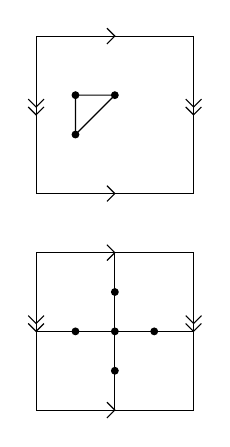
\begin{tikzpicture}[scale=.5]
\draw  (-2,2) rectangle (2,-2);
\draw (-2.2,0.4) -- (-2,0.2) -- (-1.8,0.4);
\draw (-2.2,0.2) -- (-2,0) -- (-1.8,0.2);
\draw (1.8,0.4) -- (2,0.2) -- (2.2,0.4);
\draw (1.8,0.2) -- (2,0) -- (2.2,0.2);
\draw (-0.2,2.2) -- (0,2) -- (-0.2,1.8);
\draw (-0.2,-1.8) -- (0,-2) -- (-0.2,-2.2);
\fill (0,0.5) circle[radius=.1];
\fill (-1,-0.5) circle[radius=.1];
\fill (-1,0.5) circle[radius=.1];

\draw  (-2,-3.5) rectangle (2,-7.5);
\draw (-2.2,-5.1) -- (-2,-5.3) -- (-1.8,-5.1);
\draw (-2.2,-5.3) -- (-2,-5.5) -- (-1.8,-5.3);
\draw (1.8,-5.1) -- (2,-5.3) -- (2.2,-5.1);
\draw (1.8,-5.3) -- (2,-5.5) -- (2.2,-5.3);
\draw (-0.2,-3.3) -- (0,-3.5) -- (-0.2,-3.7);
\draw (-0.2,-7.3) -- (0,-7.5) -- (-0.2,-7.7);
\fill (1,-5.5) circle[radius=.1];
\fill (-1,-5.5) circle[radius=.1];
\fill (0,-5.5) circle[radius=.1];
\fill (0,-6.5) circle[radius=.1];
\fill (0,-4.5) circle[radius=.1];
\draw (-1,0.5) -- (-1,-0.5) -- (0,0.5) -- (-1,0.5);
\draw (-2,-5.5) -- (2,-5.5);
\draw (0,-3.5) -- (0,-7.5);
\end{tikzpicture}}
Just like we know that all planar graphs have Euler characteristic 2, the Euler characteristic of a net is only dependent on the surface. 
\begin{theorem}
Suppose that $G_1, G_2$ are two different nets for a surface $\Sigma$. Then $\chi_{G_1}(\Sigma)=\chi_{G_2}(\Sigma).$\label{thm:eulercharacteristicsurface}
\end{theorem}
One would think that this can be proved using induction, but this cannot be done easily-- as it is difficult to come up with what the base case should be (remember, the statement is only true for nets.) Instead, we use a ``common refinement'' argument, which is a little bit like an induction argument done in reverse. \\
To prove this, we need a lemma.
\begin{lemma}
Suppose that $G$ is a topological minor of $H$. Furthermore, suppose that $H$ gives a net of $\Sigma$, and that $G$ drawn as a topological minor of $H$ also gives a net of $\Sigma$. Then $\chi_G(\Sigma)=\chi_H(\Sigma)$. 
\end{lemma}
\begin{proof}
First, we show that if $G\subset H$, and they are both nets, that  $\chi_G(\Sigma)=\chi_H(\Sigma)$. This essentially follows from the proof of \ref{thm:eulersformula}. Between $G$ and $H$ there is a sequence of subgraphs $G_1\subset G_2\subset \ldots\subset  G_k=H$, where each $G_i$ and $G_{i+1}$ differ by
\begin{itemize}
\item The addition of an edge and a vertex, 
\item The addition of an edge and a face. 
\end{itemize}
In either case, the Euler characteristic of $G_i$ and $G_{i+1}$ are the same, so we have that $\chi_G(\Sigma)=\chi_H(\Sigma)$.\\
The second thing we need to show is that if $G'$ is a subdivision of $G$, then they have the same Euler Characteristic. A quick check shows that 
\[E(G)-V(G)=E(G')-V(G'),\]
as each subdivision adds an equal number of edges and vertices to a graph. Therefore, $\chi_G(\Sigma)=\chi_{G'}(\Sigma)$. 
\end{proof}
\begin{proof}[Proof of Theorem \ref{thm:eulercharacteristicsurface}.]
Given two nets $G_1$ and $G_2$ on a surface, there is another net $H$ called the \emph{common refinement,} which contains both $G_1$ and $G_2$ as topological minors. There is a bit of topology or analysis to explicitally construct this graph, but in essence the graph is created by taking the drawings of $G_1$ and $G_2$, and creating a new graph whose vertices come from $G_1, G_2$ and the intersection points of the edges of $G_1$ and $G_2$. See \ref{fig:commonrefinement} for an example. As refinement preserves Euler characteristic, we get
\[\chi_{G_1}(\Sigma)=\chi_{H}(\Sigma)=\chi_{G_2}(\Sigma).\]
\begin{figure}
\centering
\begin{tikzpicture}
\fill[blue](8.5,-0.5) circle[radius=.1];
\fill[blue](8.5,-1.5) circle[radius=.1];
\fill[blue](7.5,-1.5) circle[radius=.1];
\fill[blue](7.5,-0.5) circle[radius=.1];

\draw  (6.5,1) rectangle (10,-2.5);
\draw[blue] (7.5,-0.5) -- (7.5,-1.5) -- (8.5,-1.5) -- (8.5,-0.5) -- (7.5,-0.5);
\fill[red](8,0.5) circle[radius=.1];
\fill[red](9.5,-1) circle[radius=.1];
\fill[red](8,-1) circle[radius=.1];
\fill[red](7,-1) circle[radius=.1];
\draw [red](7,-1) -- (8,-1) -- (8,0.5) -- (9.5,-1) -- (8,-1);
\fill[blue](0.5,-0.5) circle[radius=.1];
\fill[blue](0.5,-1.5) circle[radius=.1];
\fill[blue](-0.5,-1.5) circle[radius=.1];
\fill[blue](-0.5,-0.5) circle[radius=.1];
\draw  (-1.5,1) rectangle (2,-2.5);
\draw  (2.5,1) rectangle (6,-2.5);
\draw[blue] (-0.5,-0.5) -- (-0.5,-1.5) -- (0.5,-1.5) -- (0.5,-0.5) -- (-0.5,-0.5);
\fill[red](4,0.5) circle[radius=.1];
\fill[red](5.5,-1) circle[radius=.1];
\fill[red](4,-1) circle[radius=.1];
\fill[red](3,-1) circle[radius=.1];
\draw [red](3,-1) -- (4,-1) -- (4,0.5) -- (5.5,-1) -- (4,-1);
\fill[green] (8.5,-1) circle[radius=.1];
\fill[green] (8,-0.5) circle[radius=.1];
\fill[green] (7.5,-1) circle[radius=.1];
\draw[white]  (-2.5,2) rectangle (11.5,-3.5);
\end{tikzpicture}
\caption{A common refinement of two planar graphs.}
\label{fig:commonrefinement}
\end{figure}
\end{proof}
\begin{comment}
\subsection{Combinatorial Surfaces, and maps between surfaces}
Right now, we've been thinking of the graph and the surface as 2 different objects, where the surface gives us a structure on the graph. We'd like to make those notions the same. 
\begin{definition}
 A \emph{combinatorial surface} is a graph $G$ with a prescribed set of cycles with the following properties: 
 \begin{itemize}
  \item Each edge belongs to exactly 2 cycles
  \item There is associated dual graph given by cycles. Take a vertex and look at all of the associated faces in the dual graph. This forms a cycle. 
 \end{itemize}
 We denote the set $\Sigma=(V, E, F)$ to represent the combinatorial surfaces.  If every cycle is a 3-cycle, we say the surface is \emph{triangulated}
\end{definition}
Notice that certain nets give us surfaces; and in fact gives us a preferable way to describe the structure of a surface. \\ 
Previously, we had taken the common refinement of two different nets to prove that the Euler formula was an invariant of nets. We would like to describe that process of common subdivision but avoid using the embedding of the graph into a surface to construct this. \\
While the process of subdivision was useful for creating two graphs which were topologically the same, it's more difficult to come up with a notion of subdivision for faces. \\

\examplefigure{Consider the two graphs on the right. Both of them give planar nets for the plane, and we would like to say that one contains the other as a subdivision. Notice that we now have to think about no only subdividing the edges, but possibly the faces too. While we could come up with a list of valid operations for subdividing faces that would be difficult. It is instead to say that ``faces of one graph'' correspond to ``groups of faces in the second''}{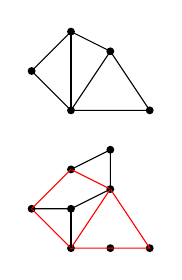
\begin{tikzpicture}[scale=.5]
\fill (0,-3.5) circle[radius=.1];
\fill (-1,-3) circle[radius=.1];
\fill (-2,-4) circle[radius=.1];
\fill (1,-5) circle[radius=.1];
\fill (-1,-5) circle[radius=.1];

\fill (0,0) circle[radius=.1];
\fill (0,-5) circle[radius=.1];
\fill (0,-2.5) circle[radius=.1];
\fill (-1,-4) circle[radius=.1];
\fill (-1,0.5) circle[radius=.1];
\fill (-2,-0.5) circle[radius=.1];
\fill (1,-1.5) circle[radius=.1];
\fill (-1,-1.5) circle[radius=.1];

\draw[red] (-1,-3) -- (-2,-4) -- (-1,-5) -- (0,-3.5) -- (-1,-3);
\draw[red] (-1,-5) -- (1,-5) -- (0,-3.5);
\draw (-1,0.5) -- (-2,-0.5) -- (-1,-1.5) -- (1,-1.5) -- (0,0) -- (-1,0.5);
\draw (-1,-1.5) -- (0,0);
\draw (-2,-4) -- (-1,-4) -- (0,-3.5) -- (0,-2.5) -- (-1,-3);
\draw (-1,-5) -- (-1,-4);
\draw (-1,-1.5) -- (-1,0.5);
\end{tikzpicture}}
Perhaps a good characterization a map between surfaces should be that it ``sends vertices to vertices, paths to paths, and contractible collections of faces to contractible collections,'' along with some information which preserves the way those faces, edges and vertices are glued together. 
\begin{definition}
Let $\Sigma= (V, E, F)$ and $\Sigma'=(V', E', F')$ be two surfaces. A \emph{map between surfaces} is a collection of linear maps
\begin{align*}
f_v:\mathcal V\to &\mathcal V'\\
f_e:\mathcal E\to &\mathcal E'\\
f_f:\mathcal F\to &\mathcal F'
\end{align*}
taking the edges of $E$ to paths in $E'$, and each face in $F$ contractible subsets of $F'$. Furthermore, these maps should respect the boundary relations 
\begin{align*}
\partial_{E'} f_e = &f_e \partial_{E}\\
\partial_{E'} f_e = &f_e \partial_{E}
\end{align*}
\end{definition}

\examplefigure{Such a map between surfaces need not be a topologically trivial map between surfaces. For instance, the map described by matching the colored faces to eachother on the right describes the ``double covering'' map of the sphere. Notice that each color in the bottom surface corresponds to 2 faces in the top surface. In Sphereical coordinates, this would correspond to the map 
\[(\theta, \phi)\mapsto (2\theta, \phi).\]
While this map is not injective, it is a valid map of surfaces. }{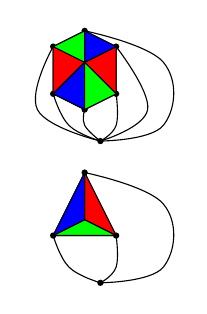
\begin{tikzpicture}[scale=.4]
\fill (-1,-3.5) circle[radius=.1];
\fill (-2,-4.5) circle[radius=.1];
\fill (-0.5,-6) circle[radius=.1];
\fill (-1,-5) circle[radius=.1];
\fill (-0.5,-10.5) circle[radius=.1];
\fill (-1,-7) circle[radius=.1];
\fill (-1,-8.5) circle[radius=.1];
\fill (-2,-3) circle[radius=.1];
\fill (-1,-2.5) circle[radius=.1];
\fill (0,-3) circle[radius=.1];
\fill (0,-4.5) circle[radius=.1];
\fill (0,-9) circle[radius=.1];
\fill (-2,-9) circle[radius=.1];
\draw (-1,-2.5) -- (-2,-3) -- (-2,-4.5) -- (-1,-5) -- (0,-4.5) -- (0,-3) -- (-1,-2.5) -- (-1,-3.5) -- (-2,-4.5);
\draw (-2,-3) -- (-1,-3.5) -- (0,-3);
\draw (-1,-5) -- (-1,-3.5) -- (0,-4.5);
\draw  plot[smooth, tension=.7] coordinates {(-1,-5) (-1,-5.5) (-0.5,-6)};
\draw  plot[smooth, tension=.7] coordinates {(-2,-4.5) (-1.5,-5.5) (-0.5,-6)};
\draw  plot[smooth, tension=.7] coordinates {(0,-4.5) (0,-5.5) (-0.5,-6)};
\draw  plot[smooth, tension=.7] coordinates {(0,-3) (1,-5) (-0.5,-6)};
\draw  plot[smooth, tension=.7] coordinates {(-2,-3) (-2.5,-5) (-0.5,-6)};
\draw  plot[smooth, tension=.7] coordinates {(-1,-2.5) (1.5,-3.5) (1.5,-5.5) (-0.5,-6)};
\draw (-1,-8.5) -- (-2,-9) -- (-1,-7) -- (0,-9) -- (-2,-9);
\draw (-1,-8.5) -- (0,-9);
\draw  plot[smooth, tension=.7] coordinates {(-2,-9) (-1.5,-10) (-0.5,-10.5)};
\draw  plot[smooth, tension=.7] coordinates {(0,-9) (0,-10) (-0.5,-10.5)};
\draw  plot[smooth, tension=.7] coordinates {(-1,-7) (1.5,-8) (1.5,-10) (-0.5,-10.5)};
\draw (-1,-8.5) -- (-1,-7);
\draw[fill=red] (-2,-3) -- (-2,-4.5) -- (-1,-3.5) -- cycle;
\draw[fill=red] (0,-3) -- (-1,-3.5) -- (0,-4.5) -- cycle;
\draw[fill=red] (-1,-7) -- (-1,-8.5) -- (0,-9) -- cycle;
\draw[fill=blue] (-1,-2.5) -- (-1,-3.5) -- (0,-3) -- cycle;
\draw[fill=blue] (-2,-4.5) -- (-1,-3.5) -- (-1,-5) -- cycle;
\draw[fill=green] (-2,-9) -- (0,-9) -- (-1,-8.5) -- cycle;
\draw[fill=green] (-1,-2.5) -- (-1,-3.5) -- (-2,-3) -- cycle;
\draw[fill=green] (-1,-3.5) -- (-1,-5) -- (0,-4.5) -- cycle;
\draw[fill=blue] (-2,-9) -- (-1,-8.5) -- (-1,-7) -- cycle;
\end{tikzpicture}}
We can use these maps between combinatorial to surfaces to when two combinatorial nets describe the same surface. 
\begin{definition}
We say that $\Sigma'$ is a subdivision of $\Sigma$ whenever there exists a combinatorial map of surfaces between them which 
\begin{itemize}
\item Is injective on vertices, 
\item Sends edges to paths whose interiors are disjoint.
\item Sends faces to collections whose interiors are disjoint. 
\end{itemize}
\end{definition}

\begin{definition}
We say that $\Sigma_1$ and $\Sigma_2$ are topologically equivalent if there exists a mutual subdivision $\Sigma'$ of both of these surfaces. 
\end{definition}
Notice that under our definition, it is not possible for two surfaces to be topologically equivalent unless they have the same Euler characteristic. This, however, is not a \emph{complete invariant}, meaning that there are surfaces $\Sigma_1$ and $\Sigma_2$ which are \emph{not equivalent,} but have $\chi(\Sigma_1)=\chi(\Sigma_2)$. \\

\examplefigure{The torus and the Klein bottle are very topologically similar surfaces. Here, we've drawn the torus on top, and the Klein bottle on the bottle. One can show that these are not the same surface; the Klein bottle is an example of a \emph{nonorientable surface.} However, the nets that they admit look very similar, making them impossible to tell apart by using the Euler characteristic (they both have Euler characteristic zero.)\\
The thing that one needs to understand in telling these two spaces apart is that that surfaces are determined more than just the nets that are drawn on them, and the incidence conditions for those nets. It is also important to consider the order of the cycles which are being glued into those nets to get an understanding for the surface.}{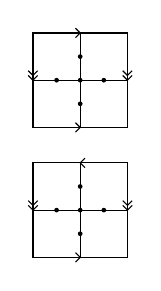
\begin{tikzpicture}[scale=.3]
\draw  (-2,-9) rectangle (2,-13);
\draw (-2.2,-10.6) -- (-2,-10.8) -- (-1.8,-10.6);
\draw (-2.2,-10.8) -- (-2,-11) -- (-1.8,-10.8);
\draw (1.8,-10.6) -- (2,-10.8) -- (2.2,-10.6);
\draw (1.8,-10.8) -- (2,-11) -- (2.2,-10.8);
\draw (0.2,-8.8) -- (0,-9) -- (0.2,-9.2);
\draw (-0.2,-12.8) -- (0,-13) -- (-0.2,-13.2);
\fill (1,-11) circle[radius=.1];
\fill (-1,-11) circle[radius=.1];
\fill (0,-11) circle[radius=.1];
\fill (0,-12) circle[radius=.1];
\fill (0,-10) circle[radius=.1];
\draw (-2,-11) -- (2,-11);
\draw (0,-9) -- (0,-13);
\draw  (-2,-3.5) rectangle (2,-7.5);
\draw (-2.2,-5.1) -- (-2,-5.3) -- (-1.8,-5.1);
\draw (-2.2,-5.3) -- (-2,-5.5) -- (-1.8,-5.3);
\draw (1.8,-5.1) -- (2,-5.3) -- (2.2,-5.1);
\draw (1.8,-5.3) -- (2,-5.5) -- (2.2,-5.3);
\draw (-0.2,-3.3) -- (0,-3.5) -- (-0.2,-3.7);
\draw (-0.2,-7.3) -- (0,-7.5) -- (-0.2,-7.7);
\fill (1,-5.5) circle[radius=.1];
\fill (-1,-5.5) circle[radius=.1];
\fill (0,-5.5) circle[radius=.1];
\fill (0,-6.5) circle[radius=.1];
\fill (0,-4.5) circle[radius=.1];

\draw (-2,-5.5) -- (2,-5.5);
\draw (0,-3.5) -- (0,-7.5);
\end{tikzpicture}}
\section{The Euler Characteristic}
\label{sec:planar:euler}
\begin{elevator}
The Euler Characteristic, determines all orientable surfaces uniquely; as a result, many facts about surfaces and their properties can be restated in terms of Euler characteristic. We relate the Euler Characteristic to curvature, handlebodies, critical points of a function on a surface and introduce homology. 
\end{elevator}
\subsection{Discrete Curvature}

In this section we prove a small result of Discrete curvature:
\begin{definition}
Let $\Sigma$ have a linear embedding into $\RR^n$, so that every edge is a line segment, and every face is contained in some 2-dimensional subspace. Then at each vertex $v$, define the \emph{curvature} 
\[\kappa(v)=2\pi \sum_{wvu} \angle wvu\]
as $2\pi$ less the measure of each angle that contains $v$ in radians. 
\end{definition}
\nomenclature{$K(\Sigma)$}{The total curvature of a surface $\Sigma$.}
\nomenclature{$\kappa(v)$}{The curvature at a point $v$.}
By taking a sum of the curvature over each vertex, we get the \emph{total curvature}, $K(\Sigma)$.\\

\examplefigure{
In the case of a standard embedding of the cube, $\kappa(v)=2\pi - 3\cdot (\pi/4)= \pi/4$. The total curvature is given by 
\begin{align*}
K(\Sigma)=&\sum_v \kappa(v)\\
=& 8 \cdot \frac{\pi}{4}=2\pi
\end{align*} }{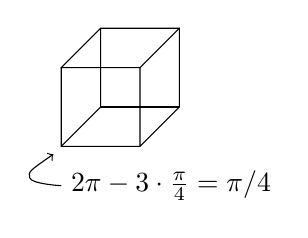
\begin{tikzpicture}[scale=.5]
\draw (-1,1) -- (-1,-1) -- (1,-1) -- (2,0) -- (2,2) -- (0,2) -- (-1,1) -- (1,1) -- (1,-1);
\draw (-1,-1) -- (0,0) -- (0,2);
\draw (2,0) -- (0,0);
\draw (2,2) -- (1,1);
\draw[<-]  plot[smooth, tension=.7] coordinates {(-1.2,-1.2) (-1.8,-1.8) (-1,-2)};
\node[right] at (-1,-2) {$2\pi-3\cdot \frac{\pi}{4}=\pi/4$};
\end{tikzpicture}}
\begin{theorem}[Discrete Gauss-Bonnet]
Let $\Sigma$ be a linearly embedded surface. Then $\kappa(\Sigma)=2\pi\chi(\Sigma)$.
\end{theorem}
\begin{proof}
Write out the sum $2\pi(V-E+F)$, and think of this as a distribution of weights onto the faces of the surface.
\begin{itemize}
\item $2\pi V$ gets distributed by adding an angle worth of weight to each of the faces containing a vertex. This leaves a surplus of $\kappa(v)$ of weight at every vertex.
\item $-2\pi E$ gets distributed by adding a weight of $-\pi$ to each face containing a specified edge.
\item $2\pi F$ gets distributed by adding a weight of $2\pi$ to each face.
\end{itemize}
Now at each face, we have a weight of $-(n-2)\pi+\sum \angle v$. But $(n-2)\pi$ is the sum of the interior angles of a face with $n$ sides, so this contribution is zero. We are left with the surplus of $\kappa(v)$ weight to distribute. So the sum of the curvatures is equal to $2\pi$ times the Euler characteristic. 
\end{proof}
\subsection{Handlebody Decomposition}
When we look at a surface, we can ``guess'' what the Euler characteristic is without actually doing an explicit computation. 
\begin{figure}[h]
\centering
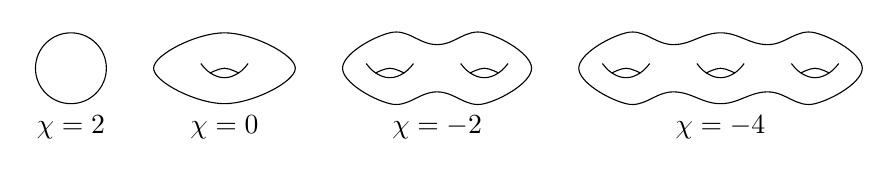
\begin{tikzpicture}[scale=.3]
\draw  plot[smooth, tension=.7] coordinates {(13,2.7) (13.4,2.3) (14,2.1) (14.6,2.3) (15,2.7)};
\draw  plot[smooth, tension=.7] coordinates {(13.4,2.3) (14,2.5) (14.6,2.3)};
\draw  plot[smooth, tension=.7] coordinates {(17,2.7) (17.4,2.3) (18,2.1) (18.6,2.3) (19,2.7)};
\draw  plot[smooth, tension=.7] coordinates {(17.4,2.3) (18,2.5) (18.6,2.3)};
\draw  plot[smooth, tension=.7] coordinates {(21,2.7) (21.4,2.3) (22,2.1) (22.6,2.3) (23,2.7)};
\draw  plot[smooth, tension=.7] coordinates {(21.4,2.3) (22,2.5) (22.6,2.3)};
\draw  plot[smooth cycle, tension=.7] coordinates {(-3,4) (-6,2.5) (-3,1) (0,2.5)};
\draw  plot[smooth, tension=.7] coordinates {(3,2.7) (3.4,2.3) (4,2.1) (4.6,2.3) (5,2.7)};
\draw  plot[smooth, tension=.7] coordinates {(3.4,2.3) (4,2.5) (4.6,2.3)};
\draw  plot[smooth, tension=.7] coordinates {(7,2.7) (7.4,2.3) (8,2.1) (8.6,2.3) (9,2.7)};
\draw  plot[smooth, tension=.7] coordinates {(7.4,2.3) (8,2.5) (8.6,2.3)};
\draw  plot[smooth, tension=.7] coordinates {(-4,2.7) (-3.6,2.3) (-3,2.1) (-2.4,2.3) (-2,2.7)};
\draw  plot[smooth, tension=.7] coordinates {(-3.6,2.3) (-3,2.5) (-2.4,2.3)};
\draw  plot[smooth cycle, tension=.7] coordinates {(2,2.5) (4,1) (6,1.5) (8,1) (10,2.5) (8,4) (6,3.5) (4,4)};
\draw  plot[smooth cycle, tension=.7] coordinates {(12,2.5) (14,1) (16,1.5) (18,1) (20,1.5) (22,1) (24,2.5) (22,4) (20,3.5) (18,4) (16,3.5) (14,4)};
\draw  (-9.5,2.5) ellipse (1.5 and 1.5);
\node at (-3,0) {$\chi=0$};
\node at (6,0) {$\chi=-2$};
\node at (18,0) {$\chi=-4$};
\node at (-9.5,0) {$\chi=2$};
\end{tikzpicture}
\caption{Some Euler Characteristics.}
\end{figure}
We want to understand how we may assemble larger surfaces from smaller ones, and figure out what the Euler characteristic of the whole is based on the Euler characteristic of the smaller parts. 
\begin{definition}Let $\Sigma_1$ and $\Sigma_2$, with nets drawn on them $G_1$ and $G_2$ respectively. Let $f_1, f_2$ be faces in $G_1$ and $G_2$, and $f_1\sim f_2$ an identifaction of their boundary cycles.  the define the \emph{connect sum of $\Sigma_1, \Sigma_2$ along $f_1\sim f_2$} to be the surface $\Sigma_1\#_{f_1\sim f_2} \Sigma_2$ defined by the net with  
\begin{itemize}
\item Vertices given by $(V(G_1)\sqcup V(G_2))/\sim$
\item Edges given by $(E(G_1)\sqcup E(G_2))/\sim$
\item Faces given by $(F(G_1)\sqcup F(G_2)\setminus \{f_1, f_2\}$
\end{itemize}
\end{definition}
Connect sum of surface can be interpreted as taking two disks on different surfaces, cutting them out, and gluing the surfaces together along the resulting boundary. See Figure \ref{fig:connectsum} for a picture of this operation. 
\begin{figure}
\centering
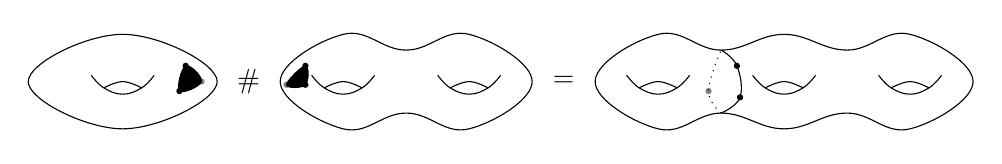
\begin{tikzpicture}[scale=.4]
\draw  plot[smooth, tension=.7] coordinates {(13,2.7) (13.4,2.3) (14,2.1) (14.6,2.3) (15,2.7)};
\draw  plot[smooth, tension=.7] coordinates {(13.4,2.3) (14,2.5) (14.6,2.3)};
\draw  plot[smooth, tension=.7] coordinates {(17,2.7) (17.4,2.3) (18,2.1) (18.6,2.3) (19,2.7)};
\draw  plot[smooth, tension=.7] coordinates {(17.4,2.3) (18,2.5) (18.6,2.3)};
\draw  plot[smooth, tension=.7] coordinates {(21,2.7) (21.4,2.3) (22,2.1) (22.6,2.3) (23,2.7)};
\draw  plot[smooth, tension=.7] coordinates {(21.4,2.3) (22,2.5) (22.6,2.3)};
\draw  plot[smooth cycle, tension=.7] coordinates {(-3,4) (-6,2.5) (-3,1) (0,2.5)};
\draw  plot[smooth, tension=.7] coordinates {(3,2.7) (3.4,2.3) (4,2.1) (4.6,2.3) (5,2.7)};
\draw  plot[smooth, tension=.7] coordinates {(3.4,2.3) (4,2.5) (4.6,2.3)};
\draw  plot[smooth, tension=.7] coordinates {(7,2.7) (7.4,2.3) (8,2.1) (8.6,2.3) (9,2.7)};
\draw  plot[smooth, tension=.7] coordinates {(7.4,2.3) (8,2.5) (8.6,2.3)};
\draw  plot[smooth, tension=.7] coordinates {(-4,2.7) (-3.6,2.3) (-3,2.1) (-2.4,2.3) (-2,2.7)};
\draw  plot[smooth, tension=.7] coordinates {(-3.6,2.3) (-3,2.5) (-2.4,2.3)};
\draw  plot[smooth cycle, tension=.7] coordinates {(2,2.5) (4,1) (6,1.5) (8,1) (10,2.5) (8,4) (6,3.5) (4,4)};
\draw  plot[smooth cycle, tension=.7] coordinates {(12,2.5) (14,1) (16,1.5) (18,1) (20,1.5) (22,1) (24,2.5) (22,4) (20,3.5) (18,4) (16,3.5) (14,4)};

\fill[gray] (15.6,2.2) node (v5) {} circle[radius=.1];
\fill (16.6,2) circle[radius=.1];
\fill (16.5,3) circle[radius=.1];
\fill[gray] (2.2,2.4) circle[radius=.1];
\fill (2.8,2.4) circle[radius=.1];
\fill (2.8,3) node (v4) {} circle[radius=.1];
\fill[gray] (-0.5,2.5) node (v3) {} circle[radius=.1];
\fill (-1.2,2.2) node (v2) {} circle[radius=.1];
\fill (-1,3) node (v1) {} circle[radius=.1];
\draw[fill=\shadinga]  plot[smooth cycle, tension=.7] coordinates {(v1) (v2) (v3)};
\draw[fill=\shadinga]  plot[smooth cycle, tension=.7] coordinates {(v4) (2.2,2.4) (2.8,2.4)};
\draw  plot[smooth, tension=.7] coordinates {(16.4,3.6)};
\draw  plot[smooth, tension=.7] coordinates {(16,3.5) (16.5,3) (16.6,2) (16,1.5)};
\draw[dotted]  plot[smooth, tension=.7] coordinates {(16,1.5) (v5) (16,3.5)};
\node at (1,2.5) {$\#$};
\node at (11,2.5) {$=$};
\end{tikzpicture}
\caption{The connect sum of 2 surfaces.}
\label{fig:connectsum}
\end{figure}
Connect sum is a operation which allows us to build surfaces out of simpler ones, and explains why we are able to ``visually'' understand what the Euler Characteristic of a surface is by visual inspection.
\begin{claim}
The Euler characteristic of the connect sum is related to the Euler charactertistic of the original components by 
\[\chi(\Sigma_1\#_{f_1\sim f_2} \Sigma_2)=\chi(\Sigma_1)+\chi(\Sigma_2)-2.\]
\end{claim}
\begin{proof}
Suppose that the boundary of $f_1$ has $k$ edges and $k$ vertices. Then we have 
\begin{align*}
V(\Sigma_1\#_{f_1\sim f_2} \Sigma_2)=&V(\Sigma_1)+V(\Sigma_2)-k\\
E(\Sigma_1\#_{f_1\sim f_2} \Sigma_2)=&E(\Sigma_1)+E(\Sigma_2)-k\\
F(\Sigma_1\#_{f_1\sim f_2} \Sigma_2)=&F(\Sigma_1)+F(\Sigma_2)-2\\
\chi(\Sigma_1\#_{f_1\sim f_2} \Sigma_2)=&\chi(\Sigma_1)+\chi(\Sigma_2)-k.
\end{align*}
\end{proof}
Notice that connect sum with a sphere does not change the topological type of a surface. The connect sum satisfies some other nice relations which tells us something about the structure of surfaces. 
\begin{claim}
 Connected Sum has the following properties:
 \begin{itemize}
  \item (Dependence on Type 1) The type of $(\Sigma_1\#\Sigma_2)$ is independent of the face used to glue the faces together
  \item (Dependence on Type 2) If $\Sigma_1\sim \Sigma_1'$ then $(\Sigma_1\#\Sigma_2)\sim (\Sigma'_1\#\Sigma_2)$
  \item (Associativity) $(\Sigma_1\#\Sigma_2)\#\Sigma_3=\Sigma_1\#(\Sigma_2\#\Sigma_3)$
  \item (Commutativity) $\Sigma_1\# \Sigma_2=\Sigma_2\#\Sigma_1$
  \item (Identity) If $\chi(\Sigma)=2$, then $\Sigma\#\Sigma'=\Sigma'$
  \item (Grading) Define the \emph{Barred Euler Characteristic} $\bar\chi(\Sigma)=\chi(\Sigma)-2$. Then $ \bar\chi(\Sigma_1\# \Sigma_2)= \bar\chi(\Sigma_1)+\bar\chi(\Sigma_2). $ \footnotemark
 \end{itemize}
 In particular, the first 5 statements tell us that homeomorphism types of surfaces form an \emph{graded monoid}, and the \emph{Barred Euler Characteristic} is a homomorphism to $\Z$.    
\end{claim}
\footnotetext{This is not a real thing, but it will be useful for this proof. }
This monoid property can be shown to be \label{proj:classification} the only data that one needs to know about surfaces. We won't prove this in class, but it's a historical theorem in the study of topology. \project
\begin{theorem}[Classification of Surfaces]
 The Sphere, Torus and Projective Plane generate the monoid of surfaces. In fact this monoid is $\langle T, P \;|\; PT=PPP, PT=TP\rangle. $
\end{theorem}
The classification of surfaces is remarkable, as we accessible  classifications of topological manifolds if they have dimension 0, 1, or 2.  In dimension 3, one must use a trick called ``geometrization'' to classify the manifolds, (which is really hard!) In dimensions 5 and above, manifolds can be classified (smoothly) using a a technique called surgery. Dimension 4 can be topologically attacked by using the tool of surgery, but smoothly cannot; techniques to understand the smooth structure of 4 manifolds are still an area of open research. 

\subsection{Morse Theory}
We're going to take a bit of a turn to talk about some inspiration on how we will solve this problem. \\
\textfigure{Morse theory is a technique taken from differential geometry used to study the topology of shapes. The basic idea is this: take a topological shape,  and look at the points where the tangent plane to the space is parallel to the ground. Let's call these points the \emph{critical points} of the space. For instance,  if we take this lima-bean shaped sphere,  we have 4 critical points. }{
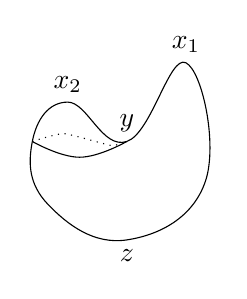
\begin{tikzpicture}[scale=1]
		\draw plot [smooth cycle, tension =.75] coordinates {(0, .75)(-1, 1.2)(-1.2, 2)(-.75, 2.5)(0, 2)(.75, 3)(1, 1.5) };
		\draw plot [smooth, tension =.75] coordinates {(-1.2, 2)(-.6, 1.8)(0, 2)};
		\draw[dotted] plot [smooth, tension =.3] coordinates {(-1.2, 2)(-.8, 2.1)(-.2, 1.95)(0, 2)};
		\draw (0, .75) node[below] {$z$};
		\draw (0, 2) node[above] {$y$};
		\draw (.75,  3) node[above] {$x_1$};
		\draw (-.75, 2.5) node[above] {$x_2$};
\end{tikzpicture}}
Now imagine at each of these critical points,  you were to drop a glob of different coloured paint,  and watch it roll down the surface of the shape. For instance,  if we were to drop blue paint at $x_1$,  and red paint at $x_2$, and opaque white paint at $x_2$,  and black paint at $z$ we would have this:
\[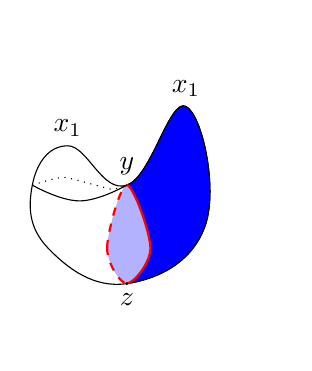
\begin{tikzpicture}[scale=1]
		\draw plot [smooth cycle, tension =.75] coordinates {(0, .75)(-1, 1.2)(-1.2, 2)(-.75, 2.5)(0, 2)(.75, 3)(1, 1.5) };
		\begin{scope}
			\clip  (0, 0)rectangle (2, 4);
			\draw[fill=blue] plot [smooth cycle, tension =.75] coordinates {(0, .75)(-1, 1.2)(-1.2, 2)(-.75, 2.5)(0, 2)(.75, 3)(1, 1.5) };
		\end{scope}
		\begin{scope}
			\clip  (0, 2)rectangle (.74, 4);
			%\draw[green,  thick] plot [smooth cycle, tension =.75] coordinates {(0, .75)(-1, 1.2)(-1.2, 2)(-.75, 2.5)(0, 2)(.75, 3)(1, 1.5) };
		\end{scope}
		\begin{scope}
			\clip  (0, 0)rectangle (.74, 4);
			\draw[red, thick,  fill =blue!30] plot [smooth cycle, tension =.55] coordinates {(0, .75)(-.25, 1.2)(0, 2) (.3, 1.2)};
		\end{scope}
		\begin{scope}
			\clip  (0, 0)rectangle (-.74, 4);
			\draw[red, dashed,  thick , fill =blue!30] plot [smooth cycle, tension =.55] coordinates {(0, .75)(-.25, 1.2)(0, 2) (.3, 1.2)};
		\end{scope}
		\draw plot [smooth, tension =.75] coordinates {(-1.2, 2)(-.6, 1.8)(0, 2)};
		\draw[dotted] plot [smooth, tension =.3] coordinates {(-1.2, 2)(-.8, 2.1)(-.2, 1.95)(0, 2)};
		\draw (0, .75) node[below] {$z$};
		\fill (0, .75) circle[radius=.02];
		\draw (0, 2) node[above] {$y$};
		\draw (.75,  3) node[above] {$x_1$};
		\draw (-.75, 2.5) node[above] {$x_1$};
\end{tikzpicture}\]
Morse theory makes the following observations:
\begin{itemize} 
	\item Each of the areas colored by a single flow of paint is a point,  line,  disk-- in general it is a $n$-simplex. 
	\item Each of area of point flows down to one of smaller dimension.
\end{itemize}
While to make this rigorous takes a substantial amount of differential geometry,  we can briefly outline the overall ideas. You take a function from the space $X$ to the real numbers,  called the height functions. The horizontal tangent spaces of this function are the critical points of the function. We will want to do a similar thing for our simplicial spaces.\\
In certain cases, every critical point looks locally like a maximum, a minimum, or a saddle. This can be stated rigerously by defining the \emph{index} as the number of negative eigenvalues of the Hessian at a critical point. In our example, $x_1, x_2$ have index 2, $y$ has index 1, and $z$ has index $0$. \\
Notice that the index of a critical point determines the dimension of the flow space emanating from that critical point. Each flow space is contractible, so it is reasonable to  come up with the following conjectural relationship:\\
\[\begin{tabular}{l|l|l}
Index & Dimension Flow Space & Graph Theoretic Analogue\\ \hline
2 & 2& Face\\
1& 1& Edge\\
0 & 0 & Vertex
\end{tabular} \]
While we cannot assemble graphs from the morse function, we can define their Euler characteristics. 
\begin{theorem} Let $f:\Sigma\to \RR$ be a function with non-degenerate critical points. Define the \emph{Euler characteristic of $f$} to be 
\[\chi_f(\Sigma)\sum_{x\in \Crit(f)} (-1)^{\ind(f)}.\]
This is no different than the Euler Characteristic of $\Sigma,$
\[\chi_f(\Sigma)=\chi(\Sigma).\]
\end{theorem}
We won't be able to prove the full differential geometry version of this theorem, as we don't have access to the machinery of differential geometry and analysis necessary to make this rigerous. 
\subsubsection{Discrete Morse Functions}
However, there is a discrete analogue of Morse functions which draws much of it's philosophy from the smooth construction.\label{proj:morsetheory} \project This theory works in the general setting of simplicial complexes, but here we will restrict ourselves to the case of surfaces. The full theory of Discrete Morse Functions, and their associated homology theory, is fleshed out in \cite{forman2002user}. 
\begin{definition}
Let $\Sigma$ be a triangulated surface. Write $\Delta(\Sigma)= V\cup E\cup F$. $\Delta(\Sigma)$ comes with a \emph{partial order} given by $v<e<f$ whenever $v$ is a vertex contained in the edge $e$, and $e<f$ whenever $e$ is an edge contained in the face $f$. \\
\end{definition}
If $\alpha< \beta \in \Delta$ are two simplices without an intermediary $\alpha<\gamma<\beta$, then we say that $\alpha$ is a \emph{facet} of $\beta$ and write $\alpha\lessdot\beta$. \\
The kind of functions which mimic those describing paint flows are \emph{discrete morse functions. } 
\begin{definition}[Discrete Morse Function]
Let $\Sigma$ be a triangulated surface. A \textbf{discrete Morse function} for $\Sigma$ is a function $f: \Delta(\Sigma)\to \RR$ such that for every simplex $\alpha$,
\[|\{\beta \;|\; \beta\lessdot \alpha ,  f(\beta)\geq f(\alpha)\}|\leq 1\]
\[|\{\beta \;|\; \alpha\lessdot \beta ,  f(\alpha)\geq f(\beta)\}|\leq 1.\]
\end{definition}
The rules for a Morse function look a little bit strange, but they can be summarized with two ideas:
\begin{itemize}
\item  Most of the time, the morse function increases as you go from vertex to edge to face. If this is not the case, we have two sets,  $\{\beta \;|\; \beta\lessdot \alpha ,  f(\beta)\geq f(\alpha)\}$ the \emph{upward exception} and $\{\beta \;|\; \alpha\lessdot \beta ,  f(\alpha)\geq f(\beta)\}$ the downward exception. 
\item A Morse function is a function which has at most 1 upward exception at each simplex, and at most 1 downward exception at each simplex. 
\end{itemize}

\examplefigure{The labeling on the right gives a morse function on the sphere, with a net given by a tetrahedron. One can see that in this representation, the outside face is the ``maximum'' of the sphere, while the central function is the ``minimum'' of the morse function. Notice that the function roughly increases in value as we go from the center of the diagram to the outside of the diagram. In this example, there is a maximum and minimum, and nothing that looks like a ``saddle'' point. }{ 
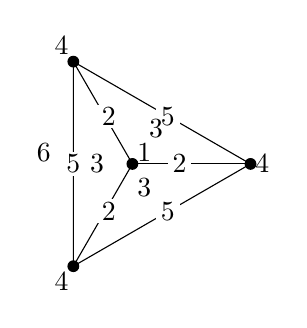
\begin{tikzpicture}[scale=.75]

\fill (0, 0) circle[radius=.1];
\fill (120:2) circle[radius=.1];
\fill (240:2) circle[radius=.1];
\fill (2,0) circle[radius=.1];
\draw (120:2) -- (-120:2) -- (0:2) -- (120:2) -- (0:0) -- (-120:2);
\draw (0:0) -- (0:2);
\fill[white]  (0.4,1) rectangle (0.8,0.6);
\fill[white]  (0.6,0.2) rectangle (1,-0.2);
\fill[white]  (-1.2,0.2) rectangle (-0.8,-0.2);
\fill[white]  (0.4,-0.6) rectangle (0.8,-1);
\fill[white]  (-0.6,1) rectangle (-0.2,0.6);
\fill[white]  (-0.6,-0.6) rectangle (-0.2,-1);
\node at (0.2,0.2) {$1$};
\node at (-0.4,0.8) {$2$};
\node at (0.8,0) {$2$};
\node at (-0.4,-0.8) {$2$};
\node at (-0.6,0) {$3$};
\node at (0.4,0.6) {$3$};
\node at (0.2,-0.4) {$3$};
\node at (0.6,-0.8) {$5$};
\node at (-1,0) {$5$};
\node at (0.6,0.8) {$5$};
\node at (-1.2,2) {$4$};
\node at (2.2,0) {$4$};
\node at (-1.2,-2) {$4$};
\node at (-1.5,0.2) {$6$};
\end{tikzpicture}}
While the assignments of numbers to the simplices seems like a good idea to imitate a Morse function,  why do we have these funny conditions?  The idea is that all simplices should have at most one higher side and be the higher face of one simplex. \\
\begin{claim}
	There always exists a Morse function $f: \Sigma\to \RR$.
\end{claim}
\begin{proof}
	Just assign $f(v)=0$, $f(e)=1$ and $f(f)=2$. 
\end{proof}
\subsubsection{Critical Points}
Under this definition of a Morse function,  what should the critical values be? In the differential geometry version,  these corresponded to places where the tangent plane lay flat. In our version,  it will be simplices that are critical. 

\begin{definition}[Critical Points]
	A simplex is called a \emph{critical point} of $f: \Delta(\Sigma)\to \RR$ if the following two conditions hold:
	\[|\{\beta \;|\; \beta\lessdot \alpha ,  f(\beta)\geq f(\alpha)\}|=0\]
\[|\{\beta \;|\; \alpha\lessdot \beta ,  f(\alpha)\geq f(\beta)\}|=0.\]
\end{definition}
The idea is that a critical (face, edge, vertex) is ``held down on all sides'' by it's boundary,  and doesn't sit atop another simplex as a face. The critical simplices are colored in Figure \ref{fig:morsecritical}

\begin{wrapfigure}{l}{5cm}
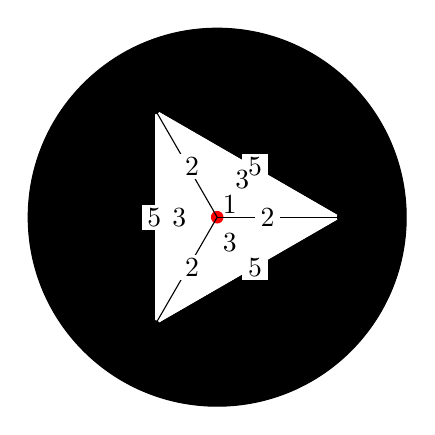
\begin{tikzpicture}[scale=.8]
\draw[fill=\highlighta]  (0,0) circle[radius=3];
\draw[fill=white] (120:2) -- (-120:2) -- (0:2) -- (120:2);
\fill[red] (0, 0) circle[radius=.1];
\fill (120:2) circle[radius=.1];
\fill (240:2) circle[radius=.1];
\fill (2,0) circle[radius=.1];
\draw (120:2) -- (-120:2) -- (0:2) -- (120:2) -- (0:0) -- (-120:2);
\draw (0:0) -- (0:2);
\fill[white]  (0.4,1) rectangle (0.8,0.6);
\fill[white]  (0.6,0.2) rectangle (1,-0.2);
\fill[white]  (-1.2,0.2) rectangle (-0.8,-0.2);
\fill[white]  (0.4,-0.6) rectangle (0.8,-1);
\fill[white]  (-0.6,1) rectangle (-0.2,0.6);
\fill[white]  (-0.6,-0.6) rectangle (-0.2,-1);
\node at (0.2,0.2) {$1$};
\node at (-0.4,0.8) {$2$};
\node at (0.8,0) {$2$};
\node at (-0.4,-0.8) {$2$};
\node at (-0.6,0) {$3$};
\node at (0.4,0.6) {$3$};
\node at (0.2,-0.4) {$3$};
\node at (0.6,-0.8) {$5$};
\node at (-1,0) {$5$};
\node at (0.6,0.8) {$5$};
\node at (-1.2,2) {$4$};
\node at (2.2,0) {$4$};
\node at (-1.2,-2) {$4$};
\node at (-2.2,0.2) {$6$};
\end{tikzpicture}
\caption{Labeling the Critical Simplices}
\label{fig:morsecritical}
\end{wrapfigure}
We now have the fundamental lemma of discrete Morse theory:

\begin{lemma}[Fundamental Lemma of DMT]
Each vertex, edge of face is only allowed to have 1 upward and/or downward exception. 
\end{lemma}
\begin{proof}
	We need only check this on the edges (as Faces may have no downward exceptions, and vertices may have no upward exceptions.)
	Suppose that $e$ is an edge with a downward exception $v$ and an upward exception $f$, so that 
	\[v\lessdot e\lessdot f\]
	\[f(v)< f(e)< f(f).\]
	Let $e'$ the other edge in the boundary of $f$ containing $v'$. This edge also satisfies
	\[v'\lessdot e\lessdot f.\]
	As $v$ has at most one downward expection, and $f$ can have at most one upward exception, 
	\[f(v)\leq f(e') \leq f(f).\]
	This contradicts our first inequality on the morse function. 
\end{proof}
Notice that if $\alpha\cdot \beta$, and $\beta$ is an downward exception for $\alpha$ then $\alpha$ is an upward exception for $\beta$. In other words, the upward and downward exceptions induce a pairing on the non-critical vertices, edges and faces of $\Sigma$. \\

\examplefigure{One way to visualize this pairing is to draw an arrow between the upward/downward exceptional pairs. This gives a ``discrete vector field'' on our space, where the only places the vector field is zero is on the critical simplices. Notice that the vector field generally points ``outward'', which is congruent with our interpretation that the gradient flow of the function should point in the increasing direction. }{
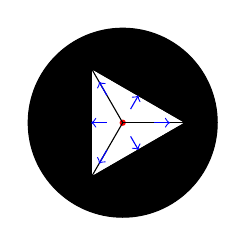
\begin{tikzpicture}[scale=.4]
\draw[fill=\highlighta]  (0,0) circle[radius=3];
\draw[fill=white] (120:2) -- (-120:2) -- (0:2) -- (120:2);
\fill[red] (0, 0) circle[radius=.1];
\fill (120:2) circle[radius=.1];
\fill (240:2) circle[radius=.1];
\fill (2,0) circle[radius=.1];
\draw (120:2) -- (-120:2) -- (0:2) -- (120:2) -- (0:0) -- (-120:2);
\draw (0:0) -- (0:2);
\draw[->,blue] (60:.5)--(60:1);
\draw[->,blue] (180:.5)--(180:1);
\draw[->,blue] (300:.5)--(300:1);
\draw[->,blue] (120:1)--(120:1.5);
\draw[->,blue] (240:1)--(240:1.5);
\draw[->,blue] (0:1)--(0:1.5);
\end{tikzpicture}}
\begin{theorem}
	Suppose $f: \Delta(\Sigma) \to \RR$  be Morse function. Then 
	$\chi(\Sigma)= \sum_{\alpha\in \Crit(f)} (-1)^{\dim(\alpha)}$
\end{theorem}
\begin{proof}
The essence of the proof is that the non-critical points are paired together in a way that causes their contributions to cancel out in the calculation of the Euler characteristic. As a computation:
\begin{align*}
\chi(\Sigma)=& \sum_{\alpha\in \Delta(G)}(-1)^{\dim(\alpha)}\\
=&\sum_{\alpha\in \Crit(f)} (-1)^{\dim(\alpha)} + \sum_{(\alpha \cdot \beta)\not\in \Crit(f)} (-1)^{\dim(\alpha)}+(-1)^{\dim(\beta)}\\
=&\sum_{\alpha\in \Crit(f)} (-1)^{\dim(\alpha) }+ \sum_{(\alpha \cdot \beta)\not\in \Crit(f)} (-1)^{\dim(\alpha)}+(-1)^{\dim(\alpha)+1}\\
=&\sum_{\alpha\in \Crit(f)} (-1)^{\dim(\alpha)}.
\end{align*}
\end{proof}




\subsection{Chain Complexes of Surfaces}
Notice, as before, that a net gives the structures of faces to a graph, and therefore we can define a homology theory as before:
\begin{definition}
Let $(\Sigma, G)$ be a surface with a net $G$ on it. Let $\mathcal F$ be the $\Z_2$ vector space generated on a basis of faces. Define the chain complex: 
\[ \begin{tikzcd}
\mathcal F \arrow{r}{\partial_F} & \mathcal E \arrow{r}{\partial_E} & \mathcal V  \arrow{r}{\partial_V} & 0
\end{tikzcd}\]
where $\partial_F$ is defined analogously to Definition \ref{def:planarcomplex}. \label{def:surfacecomplex}
\end{definition}
Recall that the set of faces formed a spanning set of the cycle space of a planar graph. The same is not is not true for surfaces! \\

\examplefigure{Notice in this net for the torus, there is only 1 face. However, there are 2 cycles: the one that goes meridinally around the torus, and the one that goes longitudinally. Since there are fewer faces than cycles, it is clear that they do not form a good basis for the cycle space.}{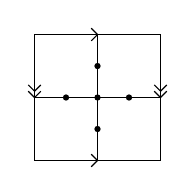
\begin{tikzpicture}[scale=.4]

\draw  (-2,-3.5) rectangle (2,-7.5);
\draw (-2.2,-5.1) -- (-2,-5.3) -- (-1.8,-5.1);
\draw (-2.2,-5.3) -- (-2,-5.5) -- (-1.8,-5.3);
\draw (1.8,-5.1) -- (2,-5.3) -- (2.2,-5.1);
\draw (1.8,-5.3) -- (2,-5.5) -- (2.2,-5.3);
\draw (-0.2,-3.3) -- (0,-3.5) -- (-0.2,-3.7);
\draw (-0.2,-7.3) -- (0,-7.5) -- (-0.2,-7.7);
\fill (1,-5.5) circle[radius=.1];
\fill (-1,-5.5) circle[radius=.1];
\fill (0,-5.5) circle[radius=.1];
\fill (0,-6.5) circle[radius=.1];
\fill (0,-4.5) circle[radius=.1];

\draw (-2,-5.5) -- (2,-5.5);
\draw (0,-3.5) -- (0,-7.5);
\end{tikzpicture}}
To prove that there are many ``interesting cycles'' that cannot be represented by faces, we'll start introducing the idea of \emph{homology.}
\begin{theorem}
The faces only span the cycle space if $(\Sigma, G)$ only if $\chi(\Sigma)=2.$
\end{theorem}
\begin{proof}
If the faces spanned the cycle space, we would be saying that 
\[\im \partial_F=\ker \partial_E .\]
However, there is no reason that this necessarily needs to be the case. The chain complex condition $\partial_E\circ \partial_F=0$ only tells us that 
\[\im \partial_F\subset\ker \partial_E .\]
As a result, the \emph{homology groups} 
\begin{align*}
H_V:=& \frac{\ker \partial V}{\im \partial_E}\\
H_E:=& \frac{\ker \partial E}{\im \partial_F}\\
H_F:=& \frac{\ker \partial F}{\im (0)}
\end{align*}
are always well defined. See \ref{def:homologygroups} for a more general construction of this. \\
If we can show that $H_E\neq 0$, then we will have prove than the faces do not span the cycle space. \\
\begin{lemma}
If $G$ is a net for $\Sigma$, then 
\[\dim H_V = \dim H_F =1 \].
\end{lemma}
\begin{proof}
The argument for $\dim H_V=1$ comes from the fact that the $\dim(H_V)=b_0(G)$, and we know that $G$ must be connected as it forms a net. Therefore, Claim \ref{claim:pathsindifferential} shows that $\dim(H_V)=b_0(G)=1$. \\
For $H_V$, we just need to compute the kernel of the $\partial_F$. Let $g$ be some collection of faces. Then $\partial_F(g)$ is just the edges which border that collection, and the collection only has empty border if every face is included. It follows that the only non-zero element in the kernel of $\partial_F$ is the sum of all the faces. 
\end{proof}
Using the lemma, we can show that the faces do not span the cycle space in a non-planar surface. We have that 
\begin{align*}
\chi(\Sigma)=& \dim (\mathcal V)-\dim (\mathcal E) + \dim (\mathcal F)\\
=& \dim( \im \partial_V)+ \dim (\ker \partial_V)\\
&-(\dim( \im \partial_E)+ \dim (\ker \partial_E))\\
&+\dim( \im \partial_F)+ \dim (\ker \partial_F)\\
=& \dim (\ker \partial_V)-\dim( \im \partial_E)\\
&-(\dim (\ker \partial_E)-\dim( \im \partial_F))\\
&+\dim (\ker \partial_F)\\
=&\dim(H_V)-\dim(H_E)+\dim(H_F)
\intertext{By the lemma}
=&2-\dim(H_E).
\end{align*}
We get as a result that $\dim(H_E)=2-\chi(\Sigma)$. This means that unless $\chi(\Sigma)=2$, the kernel of $\partial_E$ (the cycle space) is not spanned by the image of $\partial_F$. 
\end{proof}
\begin{corollary}
The Euler characteristic of a surface can never be greater than 2. 
\end{corollary}

\end{comment}